\chapter{Transfer Learning for Rapid Adaptation of Deep Neural Network Metamodels in Dynamic Hedging of Variable Annuities} \label{chap:project3}

\section{Introduction}

In the evolving landscape of financial markets, insurance products such as VAs have gained significant interest due to their ability to provide both investment growth and guaranteed benefits. 
Managing the risks associated with these products, especially in volatile market conditions, is a complex task that demands sophisticated financial modeling techniques. 
Traditional machine learning models often struggle to capture the intricate nonlinear relationships and temporal dependencies inherent in financial data.
To address the computational burden, metamodeling techniques have been proposed, where a simpler model approximates the outcomes of the more complex simulation. 
In particular, deep neural networks (DNNs), and specifically LSTM networks, have been employed as metamodels to predict the outcomes of the inner simulations efficiently
Chapter~\ref{chap:project2} introduces a nested simulation framework for dynamic hedging of VAs, where the inner simulation is approximated by an LSTM metamodel.
It shows that crude RNN and LSTMs are well-suited for metamodeling Monte Carlo simulation of financial time series and can capture the long-term dependencies in the data.

Despite the advantages of using DNN metamodels, a significant challenge arises when market conditions change or new VA contracts with different features are introduced. 
Retraining neural network metamodels from scratch in response to every change is computationally inefficient and time-consuming.
Moreover, financial markets are inherently dynamic, with frequent shifts in volatility, interest rates, and other risk factors~\citep{cont2001empirical}.
Therefore, it is essential to develop methods that can rapidly adapt existing metamodels to new conditions without incurring the full computational cost of retraining.
Transfer Learning offers a compelling solution to this problem by enabling the reuse of a pre-trained model on a new but related task~\citep{pan2009survey}.
In the context of DNNs, transfer learning involves leveraging the knowledge acquired during training on one dataset to improve learning performance on a different dataset~\citep{yosinski2014transferable}.
This approach can significantly reduce training time and computational resources while enhancing model generalization.
Instead of starting from scratch, a new DNN metamodel can be built on top of the pre-trained model and fine-tuned on the new data, allowing it to adapt quickly to changing market conditions and new VA contracts.

In this chapter, we explore the application of transfer learning to the dynamic hedging of VAs using RNN and LSTM metamodels.
We propose a novel transfer learning framework that accelerates the training of DNN metamodels for nested simulatiogn in a dynamic hedging problem.
Our approach involves pre-training an LSTM network on a large dataset of VA simulations and then fine-tuning it on a smaller dataset of new VA contracts.
We evaluate the performance of the transfer learning framework on a real-world dataset of VA contracts and compare it with training the LSTM network from scratch.

The rest of this chapter is organized as follows.
Section~\ref{sec3:background} provides an overview of the dynamic hedging problem for VAs and the use of LSTM networks as metamodels in a nested simulation procedure.
Section~\ref{sec3:transfer_learning} introduces the transfer learning framework for rapid adaptation of LSTM metamodels in dynamic hedging.
Section~\ref{sec3:experiments} presents the experimental setup and results, comparing the performance of transfer learning with training from scratch.
Finally, Section~\ref{sec3:conclusion} concludes the chapter and discusses future research directions.

\section{Transfer Learning in Metamodeling} \label{sec3:background}

Transfer learning (TL) is a machine learning paradigm where knowledge acquired from a source task is utilized to improve learning performance on a related target task.
We refer readers to \cite{pan2009survey} for a comprehensive survey of TL techniques and applications.
In the context of DNNs metamodeling-based simulation procedures for hedging VAs, TL involves pre-training a neural network where the simulation budget is abundant and then fine-tuning it on a smaller dataset of new contracts or market conditions.
Written on the same underlying asset, different VA contracts may share common features or exhibit similar patterns, especially temporal dependencies in the underlying financial time series.
Similarly, two VAs with the same features but based on different underlying assets may have some shared characteristics that can be leveraged to improve the learning performance of the metamodel.
By transferring knowledge from a pre-trained model to a new but related task, TL can significantly reduce the computational cost of training the metamodel on the target task.

LSTM networks are well-suited for modeling sequential data due to their ability to capture long-term dependencies.
For the application of VA risk management using metamodel-based nested simulation, LSTM networks approximate the inner simulation, i.e., the mapping from market scenarios to the scenario-wise contract losses.
In Chapter~\ref{chap:project2}, we treat metamodeling as a supervised learning problem and demonstrated that LSTM networks can effectively model this complex relationships with extensive training on a large dataset of VA simulations.
The total computational cost originates from two sources: running the standard nested simulation procedure to generate the training data and training the LSTM network on the generate dataset.
Given a new of VA contract, the above process needs to be repeated to adapt the LSTM metamodel to the new contract.
For a DNN with a large number of parameters, retraining the LSTM network from scratch can be computationally expensive.
TL offers an alternative approach to keep the previous knowledge as a foundation, thus accelerates the adaptation of the LSTM metamodel to new conditions.
Computational savings come in two forms: (1) less training time is required to fine-tune the pre-trained model on the new dataset, and (2) fewer data points are needed to achieve a good LSTM metamodel, which is particularly beneficial when the standard nested simulation procedure is costly.

In supervised learning, a \textbf{domain} $\mathcal{D}$ comprises a feature space $\mathcal{X}$ and a marginal probability distribution $F$. Correspondingly, a \textbf{task} $\mathcal{T}$ consists of a label space $\mathcal{Y}$ and a predictive function $f: \mathcal{X} \rightarrow \mathcal{Y}$ that maps input features to output labels.

A typical TL framework for supervised learning consists of the following:
\begin{itemize}
    \item   \textbf{source domain}: $\mathcal{D}_{\text{So}} = \{\mathcal{X}_{\text{So}}, F_{\text{So}}(X)\}$
    \item   \textbf{source task}: $\mathcal{T}_{\text{So}} = \{\mathcal{Y}_{\text{So}}, f_{\text{So}}(\cdot)\}$
    \item   \textbf{target domain}: $\mathcal{D}_{\text{Ta}} = \{\mathcal{X}_{\text{Ta}}, F_{\text{Ta}}(x)\}$
    \item   \textbf{target task}: $\mathcal{T}_{\text{Ta}} = \{\mathcal{Y}_{\text{Ta}}, f_{\text{Ta}}(\cdot)\}$
\end{itemize}

where $\mathcal{X}_{\text{So}}$ and $\mathcal{X}_{\text{Ta}}$ include input features derived from the outer simulation of two different VA contracts or market conditions, and $F_{\text{So}}(X)$ and $F_{\text{Ta}}(x)$ are the marginal probability distributions of the source and target domains, respectively.
In our numerical experiments, the dataset is generated by running the standard nested simulation procedure in Algorithm~\ref{alg2:standardProcedure} for a large number of VA contracts.
The input features $X$ are the risk factors, and the output labels $L$ are the contract losses at each time step.
We keep the number of features to be $240$ for both source and target domains as in Section~\ref{sec2:numerical}.
The predictive function $f_{\text{So}}$ and $f_{\text{Ta}}$ are trained to estimate outputs $L_{\text{So}}$ and $L_{\text{Ta}}$ such as contract losses in inner simulations under the source and target tasks, respectively.
TL seeks to improve the learning of the target predictive function $f_{\text{Ta}}(\cdot)$ in $\mathcal{D}_{\text{Ta}}$ by leveraging the previous training on $\mathcal{D}_{\text{So}}$ and $f_{\text{So}}(\cdot)$, particularly when $\mathcal{D}_{\text{So}} \neq \mathcal{D}_{\text{Ta}}$ or $\mathcal{T}_{\text{So}} \neq \mathcal{T}_{\text{Ta}}$.
In Chapter~\ref{chap:project2}, $\mathcal{D}_{\text{So}} = \mathcal{D}_{\text{Ta}}$ and $\mathcal{T}_{\text{So}} = \mathcal{T}_{\text{Ta}}$.

In our TL setting, both the source and target tasks involve learning a mapping from the risk factors to the VA contract losses.
For the source task, we have a dataset $\mathcal{D}_{\text{So}} = { (X_{\text{So}}^{(i)}, L_{\text{So}}^{(i)}) }{i=1}^{M_{\text{So}}}$, where $M_{\text{So}}$ is the number of training samples, i.e., the number of outer simulation paths used to generate the dataset with a standard nested simulation procedure.
$X_{\text{So}}^{(i)} \in \mathcal{X}_{\text{So}}$ and $L_{\text{So}}^{(i)} \in \mathcal{Y}_{\text{So}}$.
 
The ultimate objective is to learn a metamodel $f_{\text{Ta}}$ that predicts the VA contract losses $L_{\text{So}}$ from the scenarios $X_{\text{Ta}}$ in the form of a financial time series.
TL starts by training a metamodel $f_{\text{So}}$ on the source domain $\mathcal{D}_{\text{So}}$.
$f_{\text{So}}$ is approximated by an LSTM network $f_{\text{So}}(\cdot ; \theta_{\text{So}})$, and the parameters of the LSTM network, $\theta_{\text{So}}$ are learned by minimizing a MSE loss function on the source domain.
Then the pre-trained parameters $\theta_{\text{So}}$ to inform the learning of $f_{\text{Ta}}(\cdot ; \theta_{\text{Ta}})$ on the target domain $\mathcal{D}_{\text{Ta}}$.
The training on the target domain should encourage similarity between $\theta_{\text{So}}$ and $\theta_{\text{Ta}}$ to facilitate the transfer of knowledge.

The most common TL techniques for supervised learning include fine-tuning, layer freezing, and multi-task learning. 
These techniques can be categorized based on how they leverage pre-trained metamodels and how they encourage the similarity between $f_{\text{So}}(\cdot ; \theta_{\text{So}})$ and $f_{\text{Ta}}(\cdot ; \theta_{\text{Ta}})$.

\subsection{Fine-tuning}

Fine-tuning is a commonly used TL technique that uses the \textbf{same neural network architecture} for both the source and target tasks.
We first train the source LSTM metamodel $f_{\text{So}}(\cdot; \theta_{\text{So}})$ on $\mathcal{D}_{\text{So}}$, capturing temporal dependencies and patterns relevant to the source task. 
For the target task, we initialize $\theta_{\text{Ta}} = \theta_{\text{So}}$ and proceed to fine-tune the entire network on $\mathcal{D}_{\text{Ta}}$ using a smaller learning rate. 

\begin{algorithm}[ht!]
\caption{Fine-tuning Metamodel for a Target Task}
\begin{algorithmic}[1] \label{alg3:fineTuning}
    \STATE \textbf{Input:} source dataset $\mathcal{D}_{\text{So}} = \{(X_{\text{So}}^{(i)}, L_{\text{So}}^{(i)})\}_{i=1}^{M_{\text{So}}}$ , target dataset $\mathcal{D}_{\text{Ta}} = \{(X_{\text{Ta}}^{(i)}, L_{\text{Ta}}^{(i)})\}_{i=1}^{M_{\text{Ta}}}$, learning rate $\alpha_{\text{So}}$ and smaller learning rate $\alpha_{\text{Ta}}$.
    
    \STATE Train a LSTM metamodel $f_{\text{So}}(\cdot; \theta_{\text{So}})$ on $\mathcal{D}_{\text{So}}$:
    \begin{equation}
        \theta_{\text{So}} = \min_{\theta} \frac{1}{M_{\text{So}}} \sum_{i=1}^{M_{\text{So}}} \left( f_{\text{So}}(X_{\text{So}}^{(i)}; \theta) - L_{\text{So}}^{(i)} \right)^2
    \end{equation}

    \STATE Initialize the target metamodel parameters $\theta_{\text{Ta}}$ using the pre-trained metamodel parameters:
    \[
    \theta_{\text{Ta}} \gets \theta_{\text{So}}
    \]
    
    \STATE Fine-tune the entire LSTM model $f_{\text{Ta}}(\cdot; \theta_{\text{Ta}})$ on the target dataset $\mathcal{D}_{\text{Ta}}$ using a smaller learning rate $\alpha_{\text{Ta}}$:
    \begin{equation}
        \theta_{\text{Ta}} = \min_{\theta} \frac{1}{M_{\text{Ta}}} \sum_{i=1}^{M_{\text{Ta}}} \left( f_{\text{Ta}}(X_{\text{Ta}}^{(i)}; \theta) - L_{\text{Ta}}^{(i)} \right)^2
    \end{equation}
    
    \STATE \textbf{Output:} Final adapted LSTM metamodel $f_{\text{Ta}}(\cdot; \theta_{\text{Ta}})$ for the target task
\end{algorithmic}
\end{algorithm}

Algorithm~\ref{alg3:fineTuning} assumes that the learned sequential representations are beneficial for the target task.
Only minor adjustments are needed to adapt the metamodel to the new task, and the training process is accelerated by the pre-trained parameters.
Fine-tuning is particularly useful when the nested simulation procedures for the two VA contracts are closely related.
Only minor adjustments are needed to adapt the LSTM metamodel to the new domain.

\subsection{Layer Freezing}

In a layer freezing approach, we partition the model parameters into frozen parameters $\theta_0$ and trainable parameters $\theta_1$, such that $\theta = [\theta_0, \theta_1]$. 
Typically, $\theta_0$ are parameters of the lower layers, and $\theta_1$ are parameters of the higher layers that include the output layer.
The intuition behind layer freezing is that the lower layers capture general features that are transferable across tasks, while the higher layers are more task-specific.

\begin{algorithm}[ht!]
    \caption{Layer Freezing for Metamodel Transfer}
    \begin{algorithmic}[1] \label{alg3:layerFreezing}
        \STATE \textbf{Input:} source dataset $\mathcal{D}_{\text{So}} = \{(X_{\text{So}}^{(i)}, L_{\text{So}}^{(i)})\}_{i=1}^{M_{\text{So}}}$, target dataset $\mathcal{D}_{\text{Ta}} = \{(X_{\text{Ta}}^{(i)}, L_{\text{Ta}}^{(i)})\}_{i=1}^{M_{\text{Ta}}}$, learning rates $\alpha_{\text{So}}$ and $\alpha_{\text{Ta}}$, frozen parameters $\theta_0$, trainable parameters $\theta_1$.
        
        \STATE Train LSTM model $f_{\text{So}}(\cdot; \theta_{\text{So}})$ on $\mathcal{D}_{\text{So}}$:
        \begin{equation}
            \theta_{\text{So}} = [\theta_0, \theta_1] = \min_{\theta} \frac{1}{M_{\text{So}}} \sum_{i=1}^{M_{\text{So}}} \left( f_{\text{So}}(X_{\text{So}}^{(i)}; \theta) - L_{\text{So}}^{(i)} \right)^2
        \end{equation}
        
        \STATE Initialize the target model parameters $\theta_{\text{Ta}} = [\theta_0, \theta_1]$ using the pre-trained source model parameters $\theta_{\text{So}}$:
        \[
        \theta_{\text{Ta}} \gets \theta_{\text{So}} = [\theta_0, \theta_1]
        \]
        
        \STATE Freeze the parameters of the shared layers $\theta_0$:
        
        \STATE Fine-tune the trainable layers $\theta_1$ on the target dataset $\mathcal{D}_{\text{Ta}}$ using Algorithm~\ref{alg3:fineTuning}:
        \begin{equation}
            \theta_{\text{Ta}} = \min_{\theta_1} \frac{1}{M_{\text{Ta}}} \sum_{i=1}^{M_{\text{Ta}}} \left( f_{\text{Ta}}(X_{\text{Ta}}^{(i)}; [\theta_0, \theta_1]) - L_{\text{Ta}}^{(i)} \right)^2
        \end{equation}
        
        \STATE \textbf{Output:} Final adapted LSTM metamodel $f_{\text{Ta}}(\cdot; [\theta_0, \theta_1])$ for the target task
    \end{algorithmic}
    \end{algorithm}

\subsection{Multi-task Learning}

Multi-task learning~\citep{caruana1997multitask} refers to a machine learning paradigm where a single model is trained simultaneously on multiple related tasks.
Shared representations are learned across tasks, which can improve learning efficiency and predictive performance on each individual task with limited data.
In contrast to fine-tuning and layer freezing, multi-task learning aims to leverage learned knowledge from multiple tasks, and all tasks are trained simultaneously.

Let $\{\mathcal{T}_k\}_{k=1}^K$ represent a set of $K$ related tasks, each corresponding to a metamodeling task for a different standard nested simulation procedure.
For each task $\mathcal{T}_k$, we have a dataset $\mathcal{D}_k = { (X_k^{(i)}, L_k^{(i)}) }{i=1}^{M_k}$, where $M_k$ is the number of training samples for task $k$.
$X_k^{(i)}$ and $L_k^{(i)}$ are the features and contract loss labels for task $k$, respectively.

For our metamodeling implementation in Chapter~\ref{chap:project2}, we consider a multi-task learning framework where the LSTM layers are shared across multiple tasks, and each task has its own fully connected layer for prediction.
The network parameters are divided into shared parameters $\theta_0$ (LSTM layers) and task-specific parameters $\theta_k$ (fully connected layers for task $k$). 
As opposed to layer freezing, all parameters are trainable.
The objective function for multi-task learning is the sum of the loss functions of all tasks:

\begin{equation} 
    \min_{\theta_0, \theta_1, \dots, \theta_K} = \sum_{k=1}^K \frac{1}{M_k} \sum_{i=1}^{M_k} \left( f_i(X_k^{(i)}; \theta_0, \theta_1, \dots, \theta_K) - L_k^{(i)} \right)^2,
\end{equation}

where MSE loss function is used as the error metric, and $f_i(\cdot; \theta_0, \theta_1, \dots, \theta_K)$ is the output of the network for task $k$.
In essence, multi-task learning uses a multi-head architecture, where each task has its own output head, but the shared LSTM layers learn a common representation across tasks.
Transfer occurs through the shared LSTM layers $\theta_0$. 
These layers learn representations of temporal patterns and dependencies common to all tasks, effectively \textbf{pooling} information from multiple simulation schemes. 
The task-specific fully connected layers $[\theta_1, \dots, \theta_K]$ allow each task to capture unique characteristics not shared with other tasks.


\begin{algorithm}
    \caption{Multi-task Learning Framework for LSTM Metamodels}
    \begin{algorithmic}[1] \label{alg3:multiTaskLearning}
        \STATE \textbf{Input:} learning rate $\alpha$, set of $K$ tasks $\{\mathcal{T}_k\}_{k=1}^K$ with datasets $\mathcal{D}_k = \{(X_k^{(i)}, L_k^{(i)})\}_{i=1}^{M_k}$, task-specific parameters $\theta_k$ for each task $k$, and shared parameters $\theta_0$.
    
        \STATE Train the multi-head LSTM metamodel on all $K$ tasks simultaneously:
        \begin{equation}
            \min_{\theta_0, \{\theta_k\}_{k=1}^K} \sum_{k=1}^K \frac{1}{M_k} \sum_{i=1}^{M_k} \left( f_i(X_k^{(i)}; \theta_0, \theta_k) - L_k^{(i)} \right)^2
        \end{equation}
    
        \STATE Update both the shared parameters $\theta_0$ and task-specific parameters $\{\theta_k\}_{k=1}^K$ simultaneously using backpropagation and gradient descent with learning rate $\alpha$.
        
        \STATE \textbf{Output:} Trained multi-task LSTM metamodel $f(\cdot; \theta_0, \{\theta_k\}_{k=1}^K)$ for all $K$ tasks
    \end{algorithmic}
\end{algorithm}

Algorithm~\ref{alg3:multiTaskLearning} outlines the multi-task learning framework for LSTM metamodels for nested simulation procedures.
In Chapter~\ref{chap:project1} and Chapter~\ref{chap:project2}, we demonstrate that pooling using a metamodel can improve the computation efficiency and estimator accuracy in nested simulation procedures.
Here, pooling happens at a higher level, where information from multiple metamodels are shared to improve the learning performance on individual tasks.

Choosing appropriate simulation schemes is crucial for the success of multi-task learning. The tasks should be related to ensure that the shared layers can capture common features beneficial across tasks. 
Criteria for selecting simulation schemes include:

\begin{itemize} 
    \item   \textbf{Similarity in contract specifications:} 
            simulations involving VA contracts with similar features are likely to share underlying risk factors and policyholder behaviors. 
    \item   \textbf{Similarity in underlying assets:} 
            datasets simulated under different but related asset models can provide diverse information that enrich the shared representations.
            Datasets simulated under extreme market conditions can help the shared layers learn to hedge against tail risks.
    \item   \textbf{Temporal Dynamics:} 
            VA contracts with comparable maturity and rebalance frequency can help the shared layers learn temporal dependencies consistent across tasks. 
\end{itemize}

Suppose we aim to develop an LSTM metamodel for a GMWB contract under a stochastic volatility asset model, but we have limited data for this simulation scheme. 
For multi-task learning, we can select related nested simulation simulation procedures with relatively abundant data, such as:

\begin{itemize} 
    \item GMMB contracts under stochastic volatility models. 
    \item GMWB contracts under the Black-Scholes model. 
    \item GMWB contracts under stochastic volatility models with different parameters.
\end{itemize}

These tasks share similarities in contract features and market dynamics, enabling the shared LSTM layers to learn relevant temporal patterns applicable to the target task.
Furthermore, if a new but similar task is introduced, fine-tuning, layer freezing, and multi-task learning can be combined to leverage the pre-trained model effectively.
More specfically, the shared layers can be frozen, and the task-specific layers for a similar task in the training set can be fine-tuned on the new task.
This shared knowledge helps the model generalize better on a target task, as the LSTM layers have been exposed to a wider variety of patterns and dynamics.

\subsection{Rapid Adaptation of LSTM Metamodels} \label{sec3:transfer_learning}

In this section, we propose a TL framework for rapid adaptation of LSTM metamodels in dynamic hedging of VAs.
The goal is to leverage the knowledge acquired during training on a large dataset of VA simulations to improve the learning performance on a smaller dataset of new VA contracts.


\begin{algorithm}
    \caption{Transfer Learning Framework for LSTM Metamodels: Combining Fine-tuning, Layer Freezing, and Multi-task Learning}
    \begin{algorithmic}[1] \label{alg3:combined}
        \STATE \textbf{Input:} Set of $K$ tasks $\{\mathcal{T}_k\}_{k=1}^K$, with datasets $\mathcal{D}_k = \{(X_k^{(i)}, L_k^{(i)})\}_{i=1}^{M_k}$ for each task $k$, target dataset $\mathcal{D}_{\text{Ta}}$, learning rate $\alpha_{\text{So}}$ and $\alpha_{\text{Ta}}$, shared parameters $\theta_0$, task-specific parameters $\theta_k$ for each task $k$.
        
        \STATE \textbf{Multi-task learning:} define shared LSTM layers $\theta_0$ and task-specific fully connected layers $\theta_k$ for each task $k$. The LSTM layers are shared across all tasks $\{\mathcal{T}_k\}_{k=1}^K$.
        
        \STATE Train the multi-task LSTM metamodel on all $K$ tasks simultaneously:
        \begin{equation}
            \min_{\theta_0, \{\theta_k\}_{k=1}^K} \sum_{k=1}^K \frac{1}{M_k} \sum_{i=1}^{M_k} \left( f_i(X_k^{(i)}; \theta_0, \theta_k) - L_k^{(i)} \right)^2
        \end{equation}
        
        \STATE For a related task of hedging a new VA contract, combine fine-tuning and layer freezing:

        \STATE \textbf{Layer freezing:} once the multi-task metamodel is trained, freeze the parameters of the shared LSTM layers $\theta_0$.
        
        \STATE \textbf{Fine-tuning:}  based on task similarity, initialize the target task model parameters $\theta_{\text{Ta}}$ using parameters $\theta_k$ from task $k$.
        \[
        \theta_{\text{Ta}} \gets \theta_k 
        \]
        
        \STATE Fine-tune only $\theta_{\text{Ta}}$ on the new target dataset $\mathcal{D}_{\text{Ta}}$ using a smaller learning rate $\alpha_{\text{Ta}}$:
        \begin{equation}
            \min_{\theta_{\text{Ta}}} \frac{1}{M_{\text{Ta}}} \sum_{i=1}^{M_{\text{Ta}}} \left( f_{\text{Ta}}(X_{\text{Ta}}^{(i)}; \theta_0, \theta_{\text{Ta}}) - L_{\text{Ta}}^{(i)} \right)^2
        \end{equation}
        
        \STATE \textbf{Output:} Final adapted LSTM metamodel $f_{\text{Ta}}(\cdot; \theta_0, \theta_{\text{Ta}})$ for the new VA contracts in the target task.
    \end{algorithmic}
    \end{algorithm}

Algorithm~\ref{alg3:combined} combines the strengths of Multi-task learning, layer freezing, and fine-tuning to accelerate the training of LSTM metamodels. 

\begin{itemize}
    \item \textbf{Multi-task learning} allows the shared LSTM layers to pool information across related tasks, learning generalizable representations of temporal dependencies.
    \item \textbf{Layer freezing} ensures that shared features learned from source tasks are retained when adapting to a new task, reducing the risk of overfitting to the target simulation data.
    \item \textbf{Fine-tuning} enables the task-specific layers to adapt quickly to the new task with minimal simulation cost, leveraging the pre-trained shared layers.
\end{itemize}
    
The combination of these techniques aims to significantly reduce the computational cost of training LSTM metamodels for a new but related VA contract.

\section{Numerical Experiments} \label{sec3:experiments}

In this section, we evaluate the performance of the TL framework for rapid adaptation of LSTM metamodels in dynamic hedging of VAs.
The low noise dataset generated by the standard nested simulation procedure in Section~\ref{sec2:numerical} is used to train the source LSTM metamodels.
We consider two target tasks: one with the same contract but different underlying asset model and another with different contracts but the same asset model.

Serveral datasets generated by related standard nested simulation procedures are considered as source and target tasks.
VA contract losses are simulated under geometric Brownian motion (GBM) and regime-switching GBM (RS-GBM) asset models.
The contracts include GMMB and GMWB contracts with no lapse, static lapse, and dynamic lapse features.
The source dataset is generated by running the standard nested simulation procedure for 50,000 VA contracts, while each target task consists of 2,000 new sample paths.

\begin{enumerate}
    \item   GMMB contracts under RS-GBM asset model with no lapse.
    \item   GMMB contracts under RS-GBM asset model with static lapse.
    \item   GMMB contracts under RS-GBM asset model with dynamic lapse.
    \item   GMWB contracts under RS-GBM asset model with dynamic lapse.
\end{enumerate}

From the first task to the last task, the complexity of the simulation schemes increases, and the LSTM metamodels need to adapt to the new conditions.
Similar to Chapter~\ref{chap:project2}, the true contract losses for all scenarios are approximated by the standard nested simulation procedures with 100,000 inner replications. 
The training datasets are generated on the same scenarios with 100 inner replications.
These datasets are referred to as the \textbf{true dataset} and the \textbf{training dataset}, respectively in Section~\ref{sec2:numerical}.
Hyperparameters, dropout rates, and network architectures for the LSTM metamodels are the same as the LSTM metamodel in Section~\ref{sec2:numerical}. 
Due to limited computational resources, macro replications are not feasible for the tranfer learning experiments.

\subsection{Fine-Tuning and Layer Freezing}

\begin{figure}[ht!]
    \centering
    \begin{subfigure}{0.48\textwidth}
        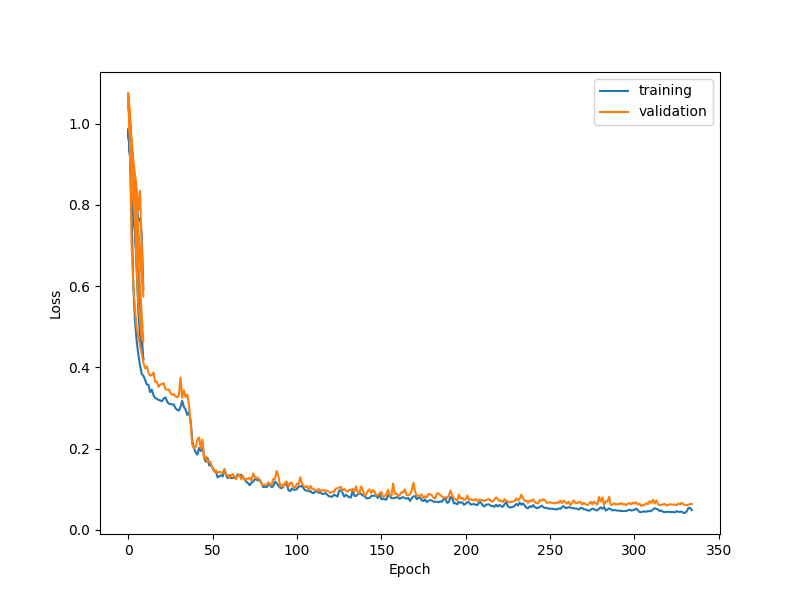
\includegraphics[width=\textwidth]{./project3/figures/figure1a.png}
        \caption{Extensive Training on Target Task} 
        \label{subfig3-1:extensive}
    \end{subfigure}\hfill
    \begin{subfigure}{0.48\textwidth}
        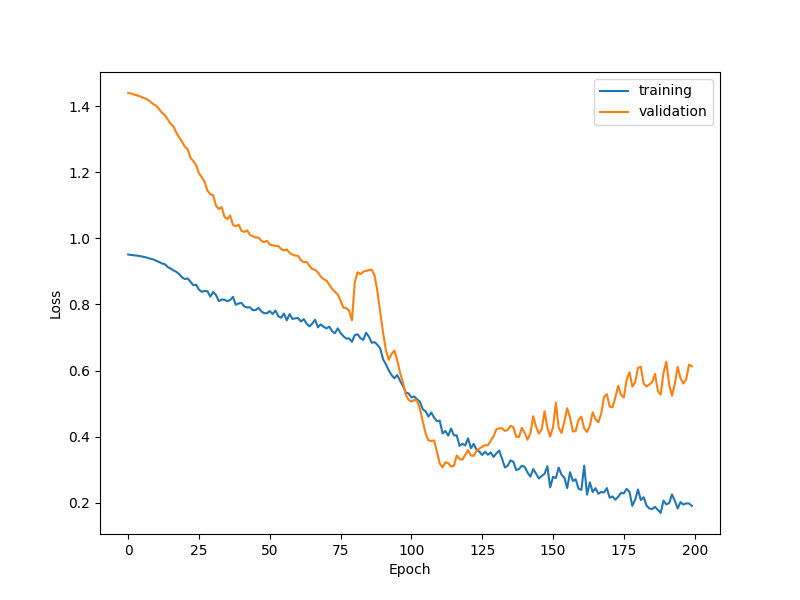
\includegraphics[width=\textwidth]{./project3/figures/figure1b.png}
        \caption{Without TL}
        \label{subfig3-1:without}
    \end{subfigure}
    \begin{subfigure}{0.48\textwidth}
        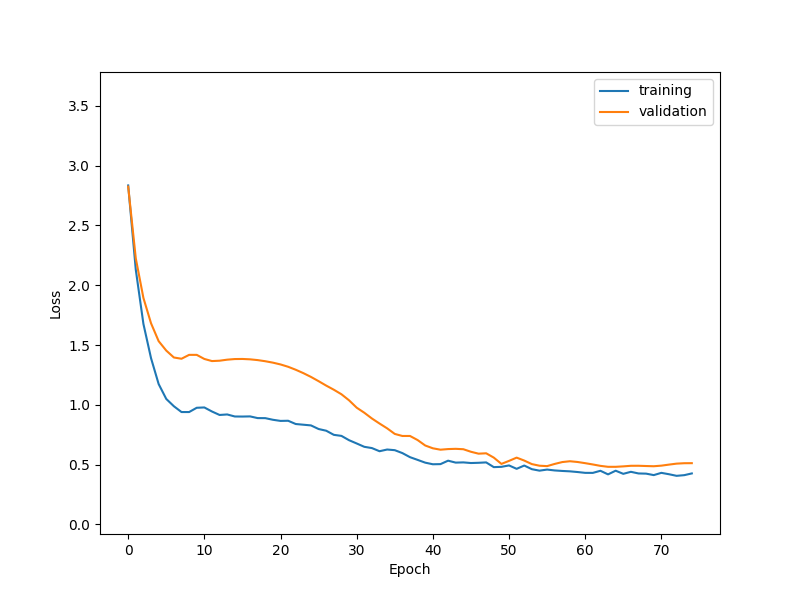
\includegraphics[width=\textwidth]{./project3/figures/figure1c.png}
        \caption{With Fine-tuning}
        \label{subfig3-1:fineTuning}
    \end{subfigure}\hfill
    \begin{subfigure}{0.48\textwidth}
        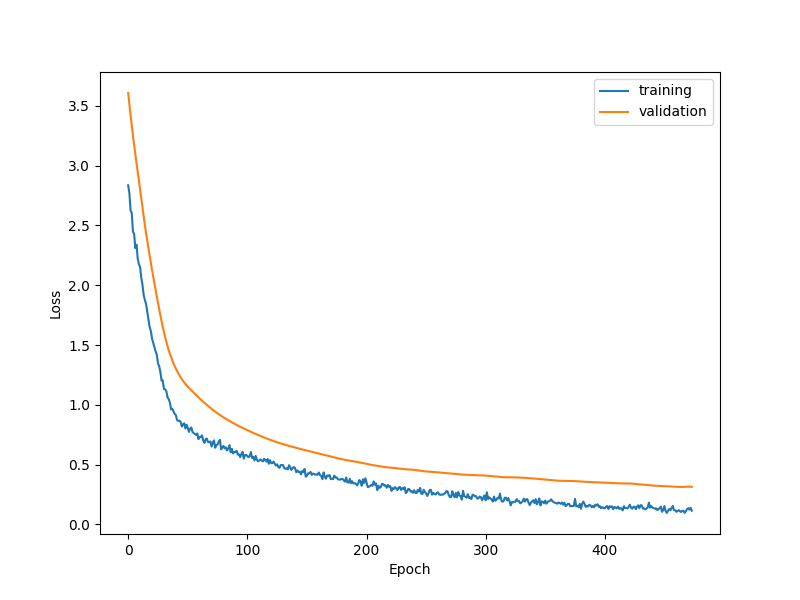
\includegraphics[width=\textwidth]{./project3/figures/figure1d.png}
        \caption{With Layer Freezing}
        \label{subfig3-1:layerFreezing}
    \end{subfigure}
    \caption{Metamodel performance on RS-GBM GMMB with static lapse}
    \label{fig3:figure1}
\end{figure}

We first compare the performance of fine-tuning and layer freezing on the target tasks.
Figure~\ref{fig3:figure1} compares the performance of LSTM metamodels on the target tasks with and without TL.
The learning history of the LSTM metamodels is shown for the target task of metamodeling GMMB contract losses on RS-GBM with static lapse.
The source task is GMMB contracts on RS-GBM with no lapse, and the target task is the same simulation scheme but with static lapse.
Figure~\ref{subfig3-1:extensive} demonstrates the performance of the LSTM metamodel trained extensively on the target task using $M_{\text{TA}} = 50,\!000$ samples, which serves as the benchmark for this study. 
The metamodel achieves a low validation error due to the availability of a large dataset.
In contrast, Figure~\ref{subfig3-1:without} presents the results of training without TL, where $M_{\text{So}} = 50,\!000$, and $M_{\text{TA}} = 2,\!000$.
This approach leads to highly unstable training dynamics, with substantial fluctuations in the validation error.
Learning without transfer leads poor generalization and extreme overfitting. 
Often, the training data is limited for a new VA contract, and such instability is particularly problematic for quick adaptation of LSTM metamodels.
Figure~\ref{subfig3-1:fineTuning} shows the results of fine-tuning a pretrained metamodel on RS-GBM with no lapse.
Fine-tuning offers noticeable improvements over training without TL by reducing the instability and lowering the validation error. 
However, despite these improvements, fine-tuning may not fully mitigate the challenges of training with a small dataset.
The fine-tuned metamodel still exhibits some fluctuations in the validation error, indicating that the model may not generalize well to new conditions.
Figure~\ref{subfig3-1:layerFreezing} presents the results of layer freezing on the same target task.
Layer freezing offers a more stable training process compared to fine-tuning, with a lower validation error and reduced fluctuations during its training.
The underlying reason is that the LSTM layers are critical for capturing general feature representations that are transferable across tasks, and freezing these layers helps prevent overfitting to the target task.
Layer freezing effectively retains useful information from the source task, while allowing the model to adapt to the new conditions in a data-efficient manner.

\subsection{Transfer to VAs with Dynamic Lapse}

\begin{figure}[ht!]
    \centering
    \begin{subfigure}{0.48\textwidth}
        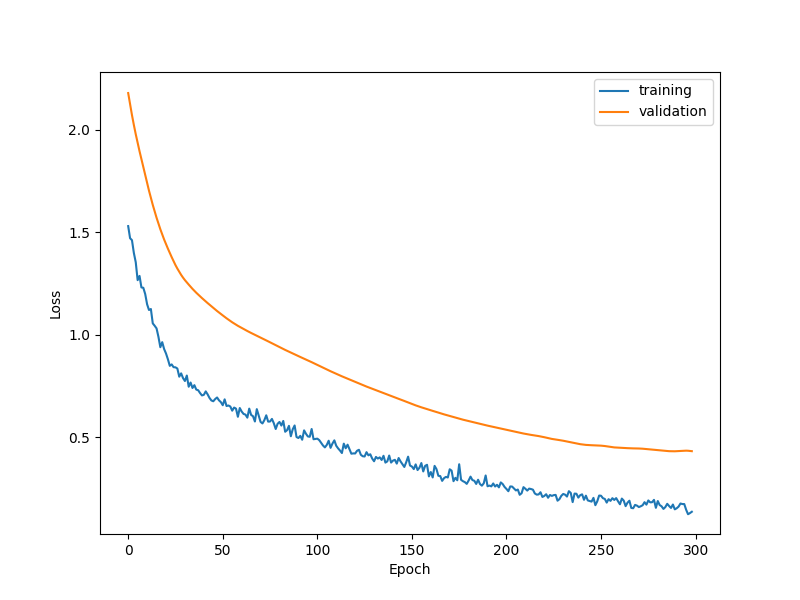
\includegraphics[width=\textwidth]{./project3/figures/figure2a.png}
        \caption{Fine-tuning from No Lapse} 
        \label{subfig3-2:fromNolapse}
    \end{subfigure}\hfill
    \begin{subfigure}{0.48\textwidth}
        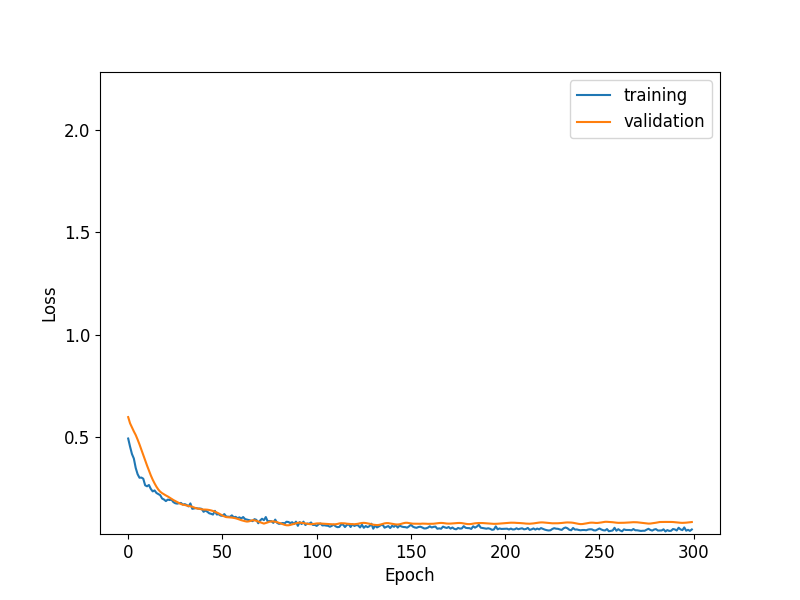
\includegraphics[width=\textwidth]{./project3/figures/figure2b.png}
        \caption{Fine-tuning from Static Lapse}
        \label{subfig3-2:fromLapse}
    \end{subfigure}
    \caption{Fine-tuned Metamodel performance on RS-GBM GMMB with dynamic lapse}
    \label{fig3:figure2}
\end{figure}

We further investigate the performance of fine-tuning on the target task of metamodeling GMMB contract losses on RS-GBM with dynamic lapse. 
The source tasks used for pretraining are GMMB contracts on RS-GBM with no lapse and static lapse, respectively. 
Figure~\ref{fig3:figure2} displays the learning curves of the LSTM metamodels fine-tuned from these two distinct source tasks.
We observe that the performance of the fine-tuned metamodel is highly dependent on the similarity between the source and target tasks.
Fine-tuning from a source task with static lapse results in faster convergence and lower validation error.
The metamodel trained on the GMMB with static lapse captures some features that are beneficial for the GMMB with dynamic lapse, which leads to a more stable training process.
In Figure~\ref{subfig3-2:fromNolapse}, the metamodel needs to learn the effect of (1) whether lapse is present and (2) whether the lapse is dynamic.
This learning process is more challenging.

The observed improvement in transferability when fine-tuning from a static lapse source task highlights the importance of selecting appropriate source tasks in TL. 
When the source task diverges significantly from the target task, the transferred metamodel may struggle to adapt to the new conditions given the limited amount of of training data.

\begin{figure}[ht!]
    \centering
    \begin{subfigure}{0.48\textwidth}
        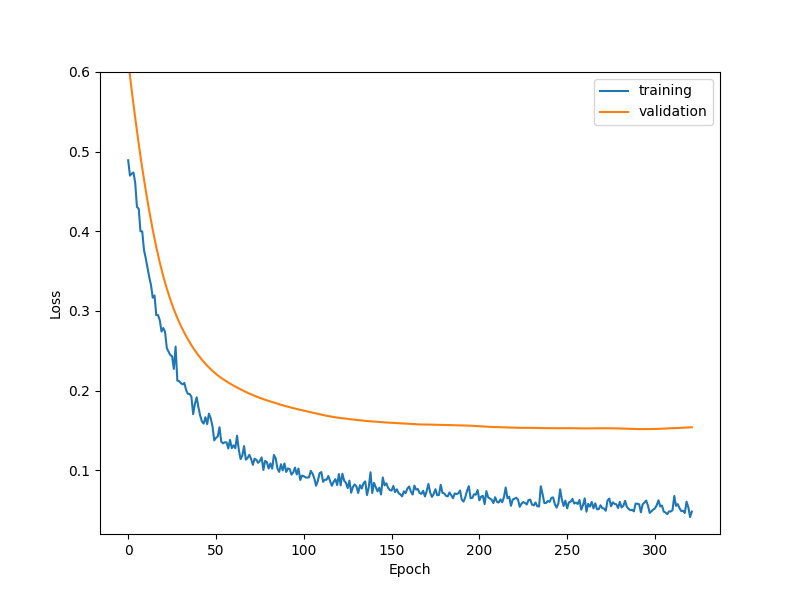
\includegraphics[width=\textwidth]{./project3/figures/figure3a.png}
        \caption{Freezing LSTM Layers} 
        \label{subfig3-3:freezeLSTM}
    \end{subfigure}\hfill
    \begin{subfigure}{0.48\textwidth}
        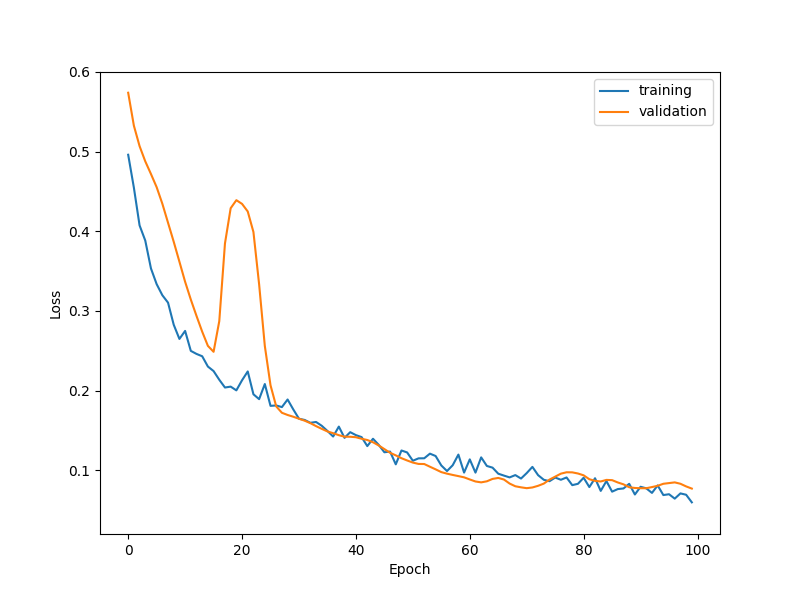
\includegraphics[width=\textwidth]{./project3/figures/figure3b.png}
        \caption{Freezing the Fully Connected Layer}
        \label{subfig3-3:freezeFC}
    \end{subfigure}
    \caption{Layer Freezing on RS-GBM GMMB with dynamic lapse}
    \label{fig3:figure3}
\end{figure}

Figure~\ref{fig3:figure3} continues the investigation of layer freezing in the task of metamodeling GMMB contract losses on RS-GBM with dynamic lapse. 
When transferring knowledge from the GMMB model with static lapse, the primary adaptation for the target task involves learning the impact of dynamic lapse.
Freezing the LSTM layers and fine-tuning only the fully connected layer results in a higher validation error, which suggests a tendency of overfitting.
This indicates that the fully connected layer struggles to adapt to the changes in the temporal dynamics introduced by dynamic lapse.
In contrast, freezing the fully connected layer and fine-tuning the LSTM layers leads to a lower validation error and better generalization. 
This can be attributed to the fact that the LSTM layers are responsible for capturing the temporal dependencies associated with dynamic lapse, while the fully connected layer remains less sensitive to shifts in the financial time series.

This experiment emphasizes the importance of choosing which layers to freeze based on the nature of the source and target tasks. 
In this case, the temporal structure of the data requires the LSTM layers to be flexible in learning new patterns related to dynamic lapse, while the fully connected layer can retain its original functionality.

\subsection{Transfer Knowledge to Other Contract Types}

When transferring knowledge from one VA contract type to another, the LSTM metamodel needs to adapt to different contract features and time series dynamics.
We consider the task of metamodeling GMWB contract losses on RS-GBM with dynamic lapse, with the source tasks being GMMB contracts on RS-GBM also with dynamic lapse.
Figure~\ref{fig3:figure4} illustrates the learning curves of the LSTM metamodels fine-tuned from the GMMB contracts to the GMWB contracts.

\begin{figure}[ht!]
    \centering
    \begin{subfigure}{0.48\textwidth}
        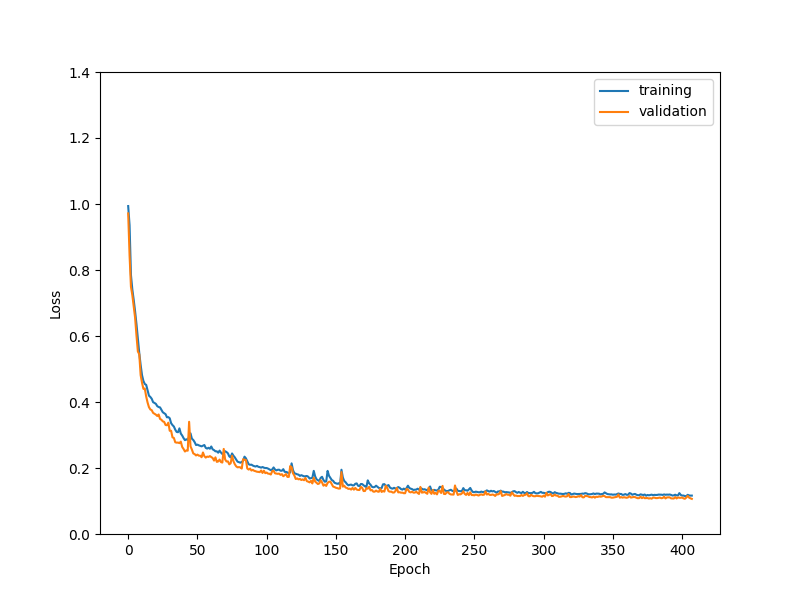
\includegraphics[width=\textwidth]{./project3/figures/figure4a.png}
        \caption{Extensive Training on Target Task} 
        \label{subfig3-4:extensive}
    \end{subfigure}\hfill
    \begin{subfigure}{0.48\textwidth}
        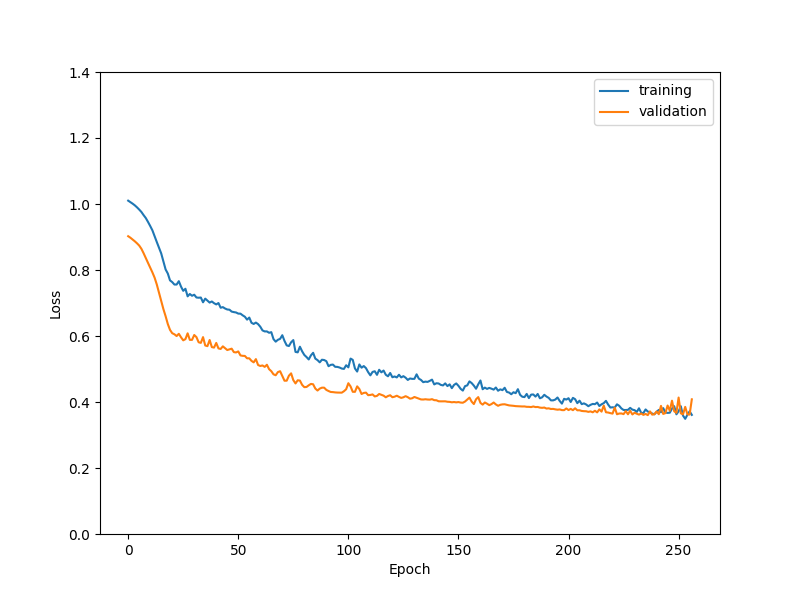
\includegraphics[width=\textwidth]{./project3/figures/figure4b.png}
        \caption{Without TL}
        \label{subfig3-4:without}
    \end{subfigure}
    \begin{subfigure}{0.48\textwidth}
        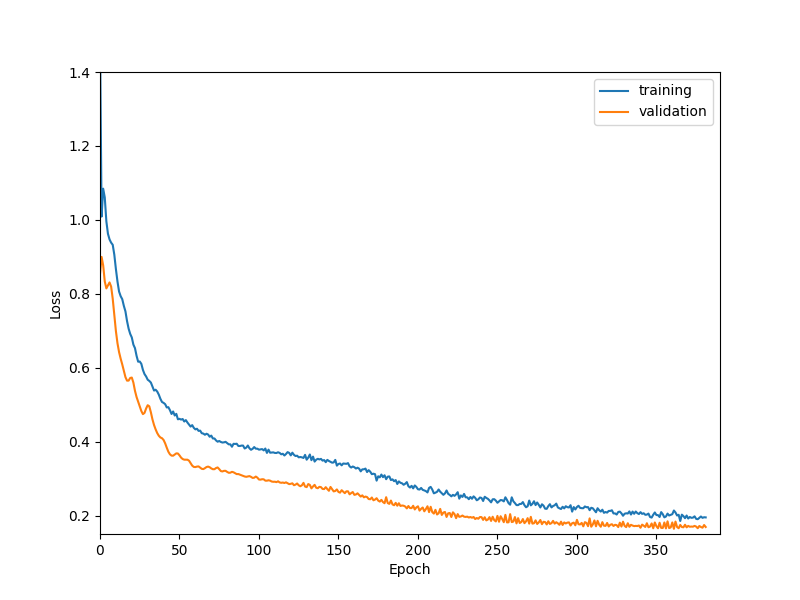
\includegraphics[width=\textwidth]{./project3/figures/figure4c.png}
        \caption{With Fine-tuning}
        \label{subfig3-4:fineTuning}
    \end{subfigure}\hfill
    \begin{subfigure}{0.48\textwidth}
        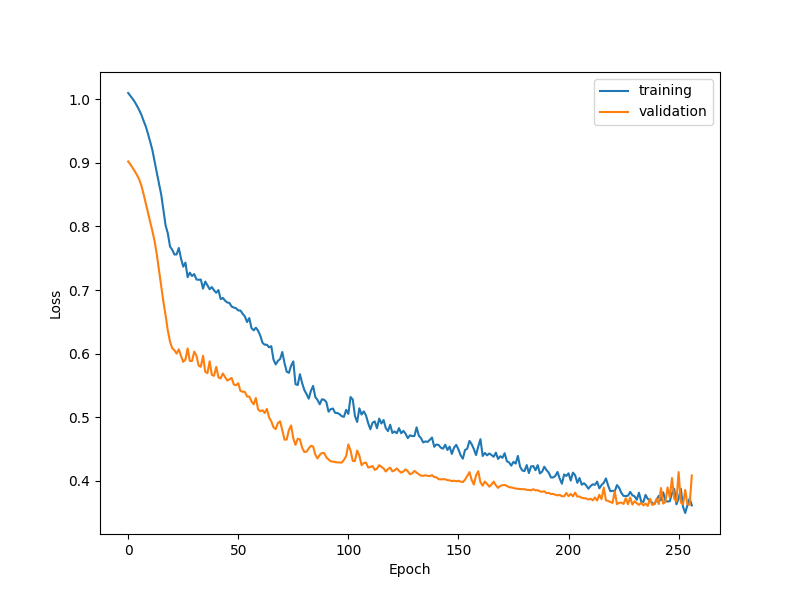
\includegraphics[width=\textwidth]{./project3/figures/figure4d.png}
        \caption{With Layer Freezing}
        \label{subfig3-4:layerFreezing}
    \end{subfigure}
    \caption{TL performance on RS-GBM GMWB with dynamic lapse}
    \label{fig3:figure4}
\end{figure}

Figure~\ref{subfig3-4:extensive} presents the performance of an extensively trained LSTM metamodel on the target task using 50,000 samples, serving as a benchmark of best metamodel performance. 
The extensively trained metamodel achieves a low validation error and demonstrates stable convergence due to having enough training samples. 
In contrast, Figure~\ref{subfig3-4:without} shows the results of training the metamodel on the target task without TL, using only 2,000 samples. The limited data leads to unstable training dynamics, with significant fluctuations in the validation error, indicating poor generalization and a tendency to overfit.

When applying fine-tuning from the GMMB source task, as depicted in Figure~\ref{subfig3-4:fineTuning}, the metamodel exhibits improved performance compared to training without TL. 
Fine-tuning results in a lower validation error and more stable convergence. 
Despite the differences between GMMB and GMWB contracts, there is still valuable information that can be transferred. 
Both the LSTM layers and the fully connected layers capture general temporal patterns and feature representations that are beneficial for the target task. 
Fine-tuning allows the metamodel to adjust all layers, facilitating better adaptation to the complexities introduced by the GMWB contracts.

However, when employing layer freezing, as shown in Figure~\ref{subfig3-4:layerFreezing}, the metamodel's performance deteriorates.
Freezing the layers trained on the GMMB contracts does not allow the metamodel to sufficiently adapt to the complexities of the GMWB contracts. 
The GMWB contracts are inherently more complex than GMMB contracts due to the guaranteed withdrawal benefits at each time step.
The complexity introduce significant changes in the time series dynamics that the metamodel needs to capture.
Freezing the LSTM layers or the fully connected layer hinders the metamodel's ability to learn these new patterns, and it leads to poor generalization and unstable error curves.

The failure of layer freezing in this context indicates that the difference between the source and target tasks is too substantial for this method to be effective. 
While layer freezing can be advantageous when the source and target tasks are closely related, it may hinder performance when the tasks diverge significantly.
In such circumstances, fine-tuning provides a better approach by allowing the metamodel to leverage transferable knowledge while adapting to the new task's specific requirements. 
Fine-tuning enables both the LSTM and fully connected layers to update their weights, capturing the complex dynamics of the GMWB contracts more effectively.

These results highlight the importance of selecting appropriate TL strategies based on the similarity between the source and target tasks. 
Even when the source and target contracts are substantially different, TL via fine-tuning can still offer performance improvements over training from scratch. 
The ability to transfer general feature representations underscores the value of TL in dynamic hedging of VAs. 
It enables more efficient training of metamodels and reduces computational burden for hedging new VA products. 
Therefore, it is still worthwhile to transfer information from GMMB contracts when developing metamodels for more complex VA contracts given limited simulation data.

\section{Conclusion} \label{sec3:conclusion}

Multi-task learning offers a robust framework for transferring knowledge across related simulation schemes in LSTM metamodeling for nested simulations. 
By sharing representations through the LSTM layers, the model can learn more generalizable features, enhancing performance on tasks with limited data. 
Careful selection of simulation schemes and thoughtful design of the network architecture are essential to maximize the benefits of MTL while mitigating potential challenges.

